In the previous sections we have seen that the second order perturbation effective Hamiltonian will contain the following terms:

\begin{itemize}
	\item Exchange interaction $J_{ij} \bs{S}_i \bs{S}_j$, arising from the kinetic hopping - kinetic hopping terms.
	\item DMI $\bs{D}_{ij} \bs{S}_i \times \bs{S}_j$, arising from the kinetic hopping - SOI hopping terms.
	\item Anisotropic or pseudodipolar interaction $\bs{S}_i \bs{\Gamma}_{ij} \bs{S}_j$, arising from the SOI hopping - SOI hopping terms.
\end{itemize}

And all these coupling factors will be renormalized by the laser field. In the cases that we obtained both exchange interaction and DMI we ignored the anisotropic interaction since it is second order in the SOI coupling constant. However, if no kinetic hopping term is allowed only the anisotropic interaction will remain (for example, the NNN interaction considered in the Kane-Mele-Hubbard model). Additionally, the symmetries of the lattice will constrain the direction the the $\bs{D}_{ij}$ vector of the DMI \cite{Moriya1960}. 

In order to summarise, we will consider the following Hamiltonian:

\begin{equation}
\hat{H} = -\sum_{\langle i,j \rangle, \sigma, \sigma'}(\delta_{\sigma, \sigma'} t_1 + \bs{\Delta}_{1,ij} \bs{\sigma}_{\sigma, \sigma'})\hat{c}_{i \sigma}^\dagger \hat{c}_{j \sigma'} - 
	\sum_{\langle \langle i,j \rangle \rangle, \sigma, \sigma'}(\delta_{\sigma, \sigma'} t_2 + \bs{\Delta}_{2,ij} \bs{\sigma}_{\sigma, \sigma'})\hat{c}_{i \sigma}^\dagger \hat{c}_{j \sigma'} + 
	\text{U}\hat{D}
\end{equation}

Which is the same we studied in section \ref{Section3HubbardSOI} plus a NNN hopping and SOI term. As before, $\bs{\Delta}_{ij}^{(n)}$ describes Rashba SOI when $\bs{\Delta}_{ij}^{(n)} = i\Delta_R^{(n)}(R_{ij}^y, -R_{ij}^x, 0)$.
The hopping amplitudes thus are:

\begin{equation}
\label{HoppHubbSOI}
t_{ij}^{\sigma \sigma'} = \begin{cases}
	(\delta_{\sigma \sigma'}t_1+\bs{\Delta}_{1,ij} \bs{\sigma}_{\sigma, \sigma'}) & \text{for } i, j \text{ nearest neighbors} \\
	(\delta_{\sigma \sigma'}t_2+\bs{\Delta}_{2,ij} \bs{\sigma}_{\sigma, \sigma'}) & \text{for } i, j \text{ next nearest neighbors} \\
	0 & \text{ otherwise}
\end{cases} \quad
\end{equation}

The effective Hamiltonian will be the same as in section \ref{Section3HubbardSOI}, with the corresponding NNN terms. This is because in second order perturbation NN hopping terms do not mix with NNN hopping terms. Thus, the effective spin Hamiltonian will be:

\begin{align}
\hat{H}_{\text{eff}}(t) = &\sum_{\langle i,j \rangle} \left\{ J_{1,ij}(t)\bs{S}_i\bs{S}_j + \bs{D}_{1,ij}(t) \bs{S}_i \times \bs{S}_j \right\} + \nonumber \\
&\sum_{\langle \langle i,j \rangle \rangle} \left\{ J_{2,ij}(t)\bs{S}_i\bs{S}_j + \bs{D}_{2,ij}(t) \bs{S}_i \times \bs{S}_j \right\}
\end{align}

Where:

\begin{align*}
J_{1,ij}(t) &= t_1^2\mathcal{M}(\alpha_{ij}, \text{U}, \omega, t) \\
\bs{D}_{1,ij}(t) &= 2it_1 \bs{\Delta}_{1,ij}\mathcal{M}(\alpha_{ij}, \text{U}, \omega, t) \\
J_{2,ij}(t) &= t_2^2\mathcal{M}(\alpha_{ij}, \text{U}, \omega, t) \\
\bs{D}_{2,ij}(t) &= 2it_2 \bs{\Delta}_{2,ij}\mathcal{M}(\alpha_{ij}, \text{U}, \omega, t)
\end{align*}

In the case $\bs{\Delta}_{1,ij} = 0$ and $\bs{\Delta}_{2,ij} = (0, 0, i \nu_{ij} \Delta)$, i.e.:

\begin{equation}
\hat{H} = - t_1\sum_{\langle i,j \rangle, \sigma} \hat{c}_{i \sigma}^\dagger \hat{c}_{j \sigma} + 
	\sum_{\langle \langle i,j \rangle \rangle, \sigma}(t_2 + i\Delta\nu_{ij}\sigma^z_{\sigma, \sigma})\hat{c}_{i \sigma}^\dagger \hat{c}_{j \sigma} + 
	\text{U}\hat{D}
\end{equation}

We recover the original Kane-Mele model with only intrinsic SOI and an additional NNN kinetic hopping term proportional to $t_1$. With this, the effective Hamiltonian will be:

\begin{equation}
\label{OtherHamsSpinModel}
\hat{H}_{\text{eff}}(t) = \sum_{\langle i,j \rangle} J_{1,ij}(t)\bs{S}_i\bs{S}_j + \sum_{\langle \langle i,j \rangle \rangle} \left\{ J_{2,ij}(t)\bs{S}_i\bs{S}_j + \bs{D}_{2,ij}(t) \bs{S}_i \times \bs{S}_j + \bs{S}_i \bs{\Gamma}_{ij}(t) \bs{S}_j \right\}
\end{equation}

Where:

\begin{align*}
J_{1,ij}(t) &= t_1^2\mathcal{M}(\alpha_{ij}, \text{U}, \omega, t) \\
J_{2,ij}(t) &= t_2^2\mathcal{M}(\alpha_{ij}, \text{U}, \omega, t) \\
\bs{D}_{2,ij}(t) &= - 2\nu_{ij} t_2 \Delta \hat{e}_z \mathcal{M}(\alpha_{ij}, \text{U}, \omega, t) \\
\bs{\Gamma}_{2,ij}(t) &= \Delta^2 \text{diag}(-1,-1,1) \mathcal{M}(\alpha_{ij}, \text{U}, \omega, t) 
\end{align*}

Now, a Hamiltonian with the form $\hat{H} = \sum_{\langle i,j \rangle} J_1 \bs{S}_i\bs{S}_j + \sum_{\langle \langle i,j \rangle \rangle} J_2\bs{S}_i\bs{S}_j$ is known as the $J_1$-$J_2$ Heisenberg model and in a 2D honeycomb lattice it exhibits N\'eel order for $J_2 < J_1 / 6$ and for $J_2 > J_1 / 6$ spin density waves (SDW) appear \cite{Mulder2010}. However, in the presence of DMI alone there will always be SDW in the plane perpendicular to $\bs{D}$ \cite{Uchida2006}. In general SDW will appear in the ground state of \ref{OtherHamsSpinModel} and the SDW wavevector will be determined by a function of the parameters of this model. Next we will show numerically that the ratio between the NN and NNN parameters can be modulated by the intensity of the field, and therefore the field can be used to control the SDW wavevector. 

We will use the time average approximation \ref{MFactorApprox0} so that we can write:

\begin{align}
J_{1,ij} &= J_{1,ij}^0  \sum_{n} \frac{\mathcal{J}_n(\alpha_{ij})^2}{1+n\frac{\omega}{\text{U}}} \\
D_{2,ij} &= D_{2,ij}^0  \sum_{n} \frac{\mathcal{J}_n(\alpha_{ij})^2}{1+n\frac{\omega}{\text{U}}}
\end{align}

Where $J_{1,ij}^0 = \frac{2t_1^2}{\text{U}}$ and $D_{2,ij}^0 = \frac{4t_2\Delta}{\text{U}}$. Now, for circularly polarized light we have $|\alpha_{ij}| = \frac{1}{\sqrt{2}}e|\vec{R}_{ij}| \frac{E_0}{\omega} = \frac{1}{\sqrt{2}}ea \frac{E_0}{\omega} \frac{|\vec{R}_{ij}|}{a} = \frac{|\vec{R}_{ij}|}{\sqrt{2}a} \mathcal{E}$:

\begin{align}
J_{1,ij} &= J_{1,ij}^0  \sum_{n} \frac{\mathcal{J}_n(\frac{1}{\sqrt{2}}\mathcal{E})^2}{1+n\frac{\omega}{\text{U}}} \\
D_{2,ij} &= D_{2,ij}^0  \sum_{n} \frac{\mathcal{J}_n(\sqrt{\frac{3}{2}}\mathcal{E})^2}{1+n\frac{\omega}{\text{U}}}
\end{align}

Therefore, $|\alpha_{ij}|$ will be $\sqrt{3}$ times bigger for NNN than for NN, and, in each case the absolute vale is independent of $i,j$.  Now, in units $\hbar=t_1=1$ we measure energy in units of $t_1$ and frequency in units of $\frac{t_1}{\hbar}$. Then, for $t_2 = 0.1$, $\Delta = 0.5$, $\text{U} = 10$ and $\omega = 6$ we obtain (ref fig). The ratio $\frac{J_{1,ij}}{D_{2,ij}}$ is plotted in (figure)

\begin{figure}
\centering
\begin{subfigure}{.5\textwidth}
  \centering
  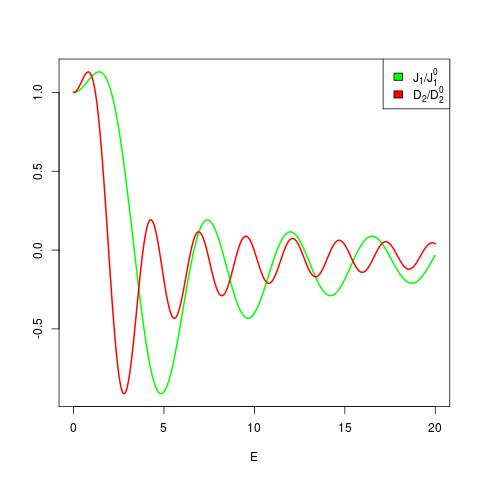
\includegraphics[width=.4\linewidth]{Chapters/NNvsNNN.jpg}
  \caption{A subfigure}
  \label{fig:sub1}
\end{subfigure}%
\begin{subfigure}{.5\textwidth}
  \centering
  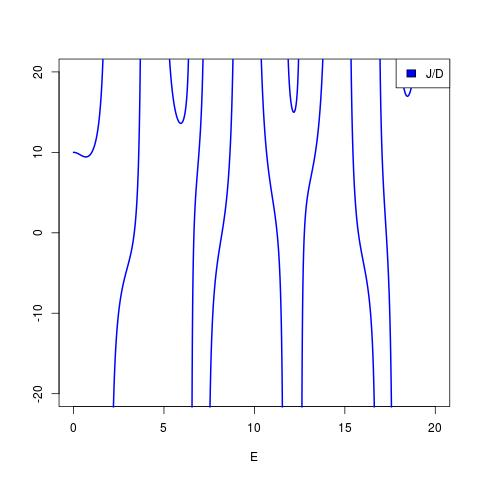
\includegraphics[width=.4\linewidth]{Chapters/ratio.jpg}
  \caption{A subfigure}
  \label{fig:sub2}
\end{subfigure}
\caption{A figure with two subfigures}
\label{fig:test}
\end{figure}




